\chapter[Thực nghiệm, kết quả và phân tích]{Thực nghiệm,\\kết quả và phân tích}
\label{chap:results}

Chương này kiểm chứng từng bước thiết kế của Chương~\ref{chap:method} theo đúng trình tự năm câu hỏi nghiên cứu ở Bảng~\ref{tab:rq}. Thay vì đưa ngay mô hình cuối cùng, các thí nghiệm được trình bày từ đơn giản đến hoàn chỉnh: (1) dữ liệu dọc và đa phương thức có giúp ích không (RQ1--RQ2); (2) tương tác song tuyến theo cặp có vượt ghép nối không (RQ3); (3) phân rã CP nén được bao nhiêu tham số và việc bỏ cặp RC có hợp lý không khi đặt cạnh bảy tổ hợp cặp cùng quy trình tham chiếu (RQ4--RQ5); và cuối cùng (4) kiểm chứng khả năng phân tầng sống còn thực tế của RC-Free qua AUC theo thời gian và đường cong Kaplan--Meier.

\section{Thiết lập huấn luyện và diễn biến hội tụ}
\label{sec:experimental-protocol}
Mọi thí nghiệm sử dụng cùng cách chia cố định theo mã người tham gia đã trình bày ở Mục~\ref{sec:data-split} (251 huấn luyện / 54 xác thực / 54 kiểm tra hậu nghiệm; tương ứng 74 / 16 / 16 biến cố), trong đó các tham số tiền xử lý chỉ khớp trên tập huấn luyện. Tập xác thực có 480 cặp so sánh hợp lệ và tập kiểm tra hậu nghiệm có 528 cặp. Loạt thăm dò đầu vào (RQ1--RQ2) chạy một lần khởi tạo; toàn bộ các so sánh kiến trúc chính và đánh giá sống còn chạy qua ba mã khởi tạo ngẫu nhiên (seed 20260727, 20260728 và 20260729), báo cáo trung bình $\pm$ độ lệch chuẩn mẫu (SD).

Do ảnh MRI 3D chiếm nhiều bộ nhớ GPU trong khi hàm mất mát Cox nhạy với cỡ lô nhỏ, quy trình huấn luyện được thiết lập như sau:
\begin{enumerate}
\item \emph{Tối ưu hóa}: Dùng AdamW \cite{loshchilov2019adamw} với tốc độ học ban đầu $10^{-4}$, weight decay $10^{-4}$, $(\beta_1,\beta_2)=(0.9,0.999)$ và cắt chuẩn gradient ở ngưỡng $1.0$ \cite{pascanu2013difficulty}.
\item \emph{Cỡ lô, tích lũy gradient và độ chính xác hỗn hợp}: Đặt cỡ lô bằng 6 người và tích lũy gradient qua 2 lô trước mỗi bước cập nhật trọng số (tập nguy cơ Cox tính riêng trên từng lô). Huấn luyện dùng FP16 \cite{micikevicius2018mixed} để giảm bộ nhớ, riêng phép tính log-sum-exp trong hàm mất mát Cox ép về FP32 để giữ ổn định số học.
\item \emph{Lấy mẫu lô hợp lệ cho Cox}: Bộ lấy mẫu phân bổ sao cho mỗi người xuất hiện đúng một lần trong mỗi vòng (42 lô/vòng) và mỗi lô luôn có ít nhất một cặp so sánh hợp lệ. Qua cả ba lần khởi tạo, toàn bộ 4032 lô huấn luyện đều hợp lệ.
\item \emph{Điều chỉnh tốc độ học và chọn mô hình}: Huấn luyện tối đa 100 vòng với \texttt{ReduceLROnPlateau} \cite{pytorchReduceLROnPlateau} theo dõi hàm mất mát Cox xác thực (giảm một nửa tốc độ học sau 5 vòng không cải thiện, mức sàn $10^{-6}$). Sau 10 vòng khởi động, dừng sớm theo dõi C-index xác thực (ngưỡng cải thiện tối thiểu 0.002, chờ 20 vòng); mô hình lưu lại là checkpoint có C-index xác thực cao nhất.
\end{enumerate}

\begin{figure}[H]
\centering
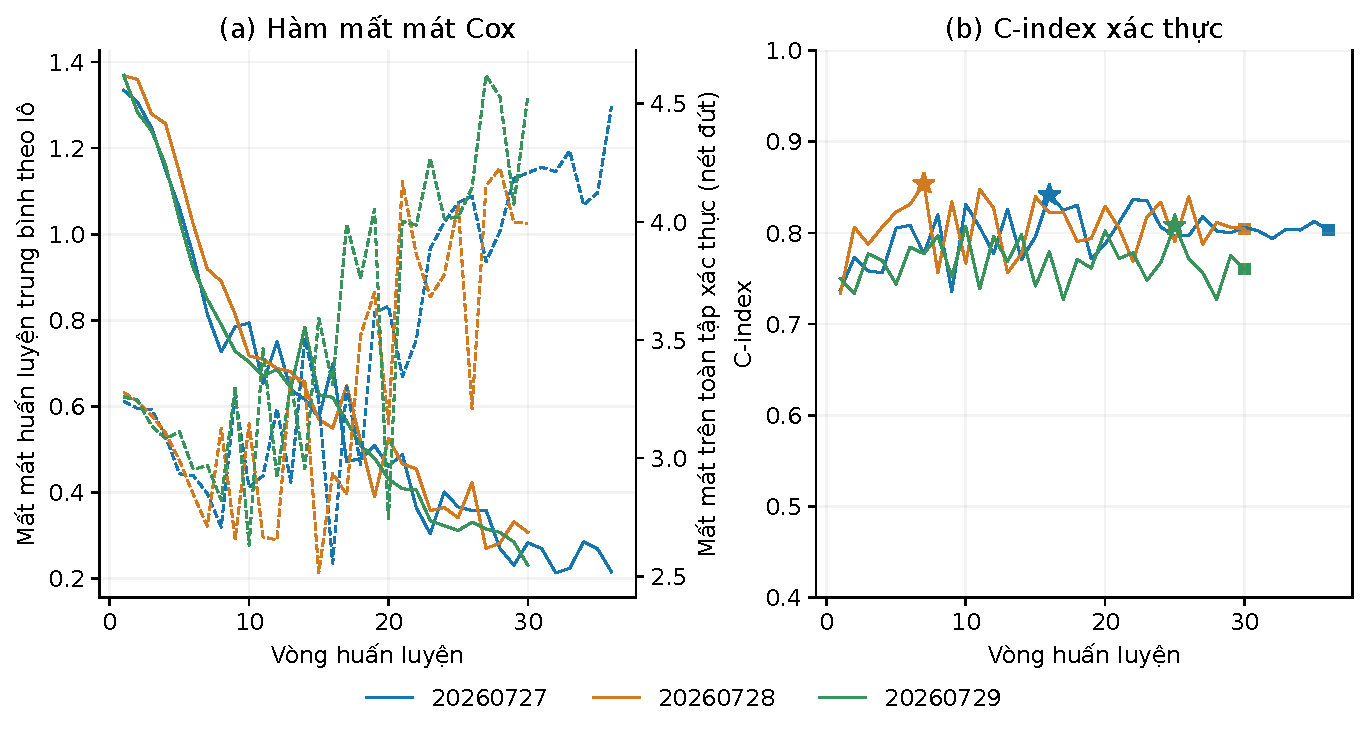
\includegraphics[width=\textwidth]{image/empirical-training.pdf}
\caption{Diễn biến huấn luyện của mô hình RC-Free qua ba lần khởi tạo}
\label{fig:empirical-training}
\captionsetup{justification=raggedright}
\caption*{Ô (a): hàm mất mát huấn luyện trung bình theo lô (đường liền, trục trái) và hàm mất mát xác thực trên toàn tập (đường đứt, trục phải). Ô (b): C-index xác thực theo từng vòng; dấu sao là mô hình được chọn, hình vuông là vòng dừng sớm.}
\end{figure}

Hình~\ref{fig:empirical-training} cho thấy trong cả ba lần chạy, hàm mất mát huấn luyện giảm đều (từ 1.33--1.37 xuống 0.22--0.31) trong khi hàm mất mát xác thực có xu hướng tăng dần (từ 3.24--3.28 lên 3.99--4.53), gợi ý hiện tượng quá khớp khi tiếp tục huấn luyện trên mẫu nhỏ. Lưu ý rằng không nên so trực tiếp trị số tuyệt đối giữa hai trục mất mát vì độ lớn hàm mất mát Cox phụ thuộc vào kích thước tập nguy cơ \cite{kvamme2019time} (tối đa 6 người mỗi lô huấn luyện so với cả 54 người trên tập xác thực). Vì mục tiêu của bài toán là xếp hạng nguy cơ, tôi chọn mô hình theo đỉnh C-index xác thực (ô b): ba lượt chạy lần lượt chọn checkpoint tại các vòng 16, 7 và 25 (đạt C-index xác thực 0.8417, 0.8542 và 0.8083) và dừng sớm ở các vòng 36, 30 và 30.

\section{Vai trò của dữ liệu dọc và đa phương thức (RQ1--RQ2)}
Bước đầu tiên của thực nghiệm kiểm tra xem việc thêm thông tin theo thời gian (nhiều lần chụp MRI) và thêm hai nguồn radiomics, lâm sàng có thực sự nâng cao khả năng xếp hạng nguy cơ hay không. Bảng~\ref{tab:exploratory} tổng hợp kết quả loạt thăm dò trên tập xác thực (seed 20260727).

\begin{table}[H]
\centering\small
\caption[So sánh cấu hình đầu vào cho RQ1--RQ2]{C-index xác thực của các cấu hình đầu vào tăng dần (seed 20260727).}
\label{tab:exploratory}
\begin{tabularx}{\linewidth}{@{}Y r@{}}
\toprule
\textbf{Cấu hình mô hình} & \textbf{C-index $\uparrow$} \\
\midrule
MRI cuối (đơn thời điểm) & 0.7333 \\
MRI dọc và T-LSTM & 0.7333 \\
MRI dọc, T-LSTM và attention & 0.7833 \\
Ghép nối ba nguồn dữ liệu (MRI + Radiomics + Lâm sàng) & \textbf{0.8125} \\
\bottomrule
\end{tabularx}
\end{table}

Kết quả cho thấy hai bước nhảy rõ rệt. Thứ nhất, chỉ dùng trạng thái cuối của T-LSTM trên ba ảnh MRI chưa vượt được mô hình chỉ dùng ảnh cuối (cùng 0.7333), nhưng khi bổ sung cơ chế attention để tổng hợp có trọng số cả ba lần khám, C-index tăng từ 0.7333 lên 0.7833 (+0.0500). Điều này cho thấy giá trị của dữ liệu dọc chỉ phát huy rõ khi mô hình được quyền cân đối đóng góp giữa các lần chụp thay vì chỉ dựa vào bước cuối. Thứ hai, khi bổ sung radiomics và dữ liệu lâm sàng bằng phép ghép nối đơn giản, C-index tăng tiếp lên \textbf{0.8125} (+0.0292 so với cấu hình chỉ dùng MRI tốt nhất). Từ cơ sở này, toàn bộ các thí nghiệm tiếp theo giữ đồng thời cả ba nguồn dữ liệu cùng T-LSTM và attention.

\section{Đối chiếu ghép nối và tương tác tích ngoài (RQ3)}
\label{sec:matched-fusion}
Khi đã giữ đủ ba nguồn đầu vào, câu hỏi tiếp theo là liệu mô hình hóa tương tác song tuyến bằng phép tích ngoài có hiệu quả hơn ghép nối đặc trưng hay không. Để cô lập đúng tác động của lớp hợp nhất, tôi cố định toàn bộ các khối còn lại (ResNet-18 3D, T-LSTM ẩn 128, attention, hàm mất mát Cox Breslow và cấu hình huấn luyện) và khởi tạo \emph{cùng trọng số ban đầu} cho các phần chung ở mỗi lần chạy (Bảng~\ref{tab:matched-fusion}).

\begin{table}[H]
\centering\small
\caption[So sánh ghép nối và tích ngoài]{C-index xác thực của ghép nối và tích ngoài khi giữ cùng trọng số khởi tạo cho các phần chung (trung bình $\pm$ SD qua ba lần chạy).}
\label{tab:matched-fusion}
\begin{tabularx}{\linewidth}{@{}Y r@{}}
\toprule
\textbf{Cấu trúc hợp nhất} & \textbf{C-index $\uparrow$} \\
\midrule
Concatenation (ghép nối) & $0.8149\pm0.0214$ \\
Full Outer-Product (tích ngoài đầy đủ) & $\mathbf{0.8285\pm0.0272}$ \\
\bottomrule
\end{tabularx}
\end{table}

Trong cùng điều kiện khởi tạo, Full Outer-Product đạt C-index xác thực trung bình \textbf{0.8285}, cao hơn mức 0.8149 của ghép nối (chênh lệch trung bình \textbf{0.0135} tính trên giá trị chưa làm tròn). Mức cải thiện này cho thấy việc biểu diễn tường minh các tích chéo giúp khai thác tốt hơn mối liên hệ giữa ba nguồn dữ liệu, tạo cơ sở để lấy Full Outer-Product làm mốc xuất phát cho hai bước tinh giản tiếp theo: nén tham số bằng phân rã CP và lược bỏ cặp tương tác dư thừa.

\section{Phân rã CP, RC-Free và đối chiếu (RQ4--RQ5)}
\label{sec:cp-results}
\label{sec:ablation-results}
\label{sec:rcfree-multiseed}
\label{sec:standardized-benchmark}
\label{sec:paper-adaptation-results}

Từ cấu trúc Full Outer-Product, tôi tiến hành hai bước đơn giản hóa nối tiếp nhau trên cùng bộ ba seed (20260727--20260729), rồi đặt mô hình chọn được cạnh quy trình tham chiếu CNN--PCA--T-LSTM.

\subsection{Mức giảm tham số nhờ phân rã CP (RQ4)}
\label{sec:computational-efficiency}
Khi chuyển từ Full Outer-Product sang Full CP, toàn bộ các bộ mã hóa, nhánh phần dư có cổng và khối thời gian được giữ nguyên; chỉ lớp song tuyến đầu của ba cặp MR, MC và RC được tham số hóa bằng CP với hạng lần lượt là 8, 8 và 4 (Bảng~\ref{tab:cpconfig}). Bảng~\ref{tab:interaction-parameters} đối chiếu số tham số ở ba phạm vi tính khác nhau.

\begin{table}[H]
\centering\small
\caption[Tham số tương tác và toàn mạng]{Số tham số của Full Outer-Product và Full CP ở ba phạm vi (gồm độ chệch).}
\label{tab:interaction-parameters}
\begin{tabularx}{\linewidth}{@{}Y r r@{}}
\toprule
\textbf{Phạm vi} & \textbf{Full Outer-Product} & \textbf{Full CP} \\
\midrule
Ba lớp song tuyến đầu & 229696 & \textbf{3712} \\
Ba khối tương tác, gồm MLP & 248608 & \textbf{22624} \\
Toàn mạng & 33760941 & \textbf{33534957} \\
\bottomrule
\end{tabularx}
\end{table}

Bảng~\ref{tab:interaction-parameters} cho thấy rõ bản chất của việc nén tham số bằng CP: ở đúng ba lớp song tuyến đầu, số tham số giảm từ 229696 xuống còn 3712, tức \textbf{giảm 98.38\%}; tính cả phần MLP phía sau của ba khối tương tác, mức giảm vẫn là \textbf{90.90\%}. Ngược lại, trên quy mô toàn mạng, mức giảm chỉ đạt khoảng 0.67\% vì xương sống ResNet-18 3D của nhánh ảnh MRI chiếm phần lớn số tham số và không thay đổi. Đổi lại mức tinh giản mạnh ở lớp tương tác, C-index xác thực trung bình của Full CP (0.8278) thấp hơn Full Outer-Product (0.8344) khoảng 0.0066 trên loạt so sánh chính (Bảng~\ref{tab:standard-bench}). Thay vì dừng ở Full CP, bước tiếp theo kiểm tra xem việc loại bỏ bớt cặp tương tác dư thừa có vừa giảm thêm tham số vừa lấy lại C-index hay không.

\subsection{So sánh bảy cấu trúc tương tác cặp và lựa chọn RC-Free (RQ5)}
\label{sec:new-topology}
Để kiểm chứng giả thuyết rằng không cần giữ đủ cả ba cặp tương tác, tôi khảo sát toàn bộ bảy tổ hợp CP có ít nhất một cặp (ba cấu hình 1 cặp, ba cấu hình 2 cặp và Full CP 3 cặp). Điểm quan trọng là \emph{mọi cấu trúc đều giữ đủ cả ba nguồn đầu vào cùng đường truyền gốc của chúng}; khác biệt duy nhất là những cặp tương tác nào được bật. Bảng~\ref{tab:new-topology} báo cáo kết quả qua ba lần khởi tạo.

\begin{table}[H]
\centering\small
\caption[So sánh bảy cấu trúc có tương tác cặp]{Số tham số toàn mạng và C-index xác thực của bảy cấu trúc CP có tương tác cặp (trung bình $\pm$ SD qua ba lần khởi tạo).}
\label{tab:new-topology}
\begin{tabularx}{\linewidth}{@{}Y c r r@{}}
\toprule
\textbf{Cấu trúc} & \textbf{Cặp / nhánh} & \textbf{Số tham số} & \textbf{C-index $\uparrow$} \\
\midrule
MR-only & 1 / 2 & 33484165 & $0.8299\pm0.0267$ \\
MC-only & 1 / 2 & 33484037 & $0.8236\pm0.0237$ \\
RC-only & 1 / 2 & 33464165 & $0.8319\pm0.0214$ \\
RC-Free (MR+MC) & 2 / 4 & 33519497 & $\mathbf{0.8347\pm0.0237}$ \\
MR-Free (MC+RC) & 2 / 4 & 33499625 & $0.8243\pm0.0249$ \\
MC-Free (MR+RC) & 2 / 4 & 33499753 & $0.8222\pm0.0156$ \\
Full CP & 3 / 6 & 33534957 & $0.8278\pm0.0250$ \\
\bottomrule
\end{tabularx}
\end{table}

Trong bảy cấu trúc, \textbf{RC-Free (MR+MC)} đạt C-index xác thực trung bình cao nhất (\textbf{0.8347}), đứng thứ hai là RC-only (0.8319). So với Full CP, bỏ cặp RC giúp giảm số nhánh phần dư từ sáu xuống bốn, \textbf{tiết kiệm 15460 tham số} và nâng C-index trung bình từ 0.8278 lên 0.8347. Xét đồng thời cả tiêu chí giữ tương tác tường minh quanh ảnh MRI lẫn hiệu quả xếp hạng và độ tinh gọn, RC-Free là lựa chọn hợp lý nhất để đưa vào phân tích sống còn.

\subsection{Đối chiếu tổng thể với quy trình tham chiếu}
Bảng~\ref{tab:standard-bench} đặt RC-Free cạnh Full Outer-Product, Full CP và bản tái lập có điều chỉnh quy trình CNN--PCA--T-LSTM của Aghajanian và cộng sự trên cùng tập xác thực.

\begin{table}[H]
\centering\small
\caption[So sánh C-index và độ phức tạp mô hình]{C-index xác thực dưới dạng trung bình $\pm$ SD qua ba lần khởi tạo. M biểu thị triệu tham số.}
\label{tab:standard-bench}
\begin{tabularx}{\linewidth}{@{}Y r r c@{}}
\toprule
\textbf{Mô hình} & \textbf{C-index $\uparrow$} & \textbf{Tham số (M)} & \textbf{Cặp/nhánh} \\
\midrule
CNN--PCA--T-LSTM (thích nghi) & $0.7417\pm0.0693$ & $33.20\text{--}33.21$ & 0 / 0 \\
Full Outer-Product (loạt chính) & $0.8344\pm0.0148$ & $33.76$ & 3 / 6 \\
Full CP Pairwise & $0.8278\pm0.0250$ & $33.53$ & 3 / 6 \\
RC-Free Pairwise & $0.8347\pm0.0237$ & $33.52$ & 2 / 4 \\
RC-Free Fixed-$\lambda$ & $0.8347\pm0.0313$ & $33.52$ & 2 / 4 \\
\bottomrule
\end{tabularx}
\end{table}


So với Full Outer-Product, RC-Free \textbf{giảm 241444 tham số} (rút từ 3 cặp / 6 nhánh xuống 2 cặp / 4 nhánh) trong khi vẫn đạt C-index trung bình cao nhất (\textbf{0.8347} so với 0.8344). Đặt cạnh quy trình tham chiếu CNN--PCA--T-LSTM ($0.7417\pm0.0693$), cả ba kiến trúc hợp nhất đa phương thức đầu-cuối đều đạt C-index cao hơn khoảng 0.086--0.093 điểm, đồng thời có độ lệch chuẩn qua ba lần khởi tạo nhỏ hơn gần ba lần (0.0148--0.0250 so với 0.0693). Kết quả này cho thấy quy trình huấn luyện đầu-cuối kết hợp bộ mã hóa tiền huấn luyện và tương tác đa nguồn mang lại cả độ chính xác xếp hạng lẫn độ ổn định vượt trội so với quy trình hai bước chỉ dùng đặc trưng ảnh nén qua PCA.

\section{Phân tích sống còn của RC-Free}
\label{sec:posthoc-test}
\label{sec:survival-results}
Với cấu trúc RC-Free đã chọn, phần này kiểm chứng chất lượng điểm nguy cơ $\eta_i$ trên cả tập xác thực (đánh giá chính) và tập kiểm tra hậu nghiệm theo hai góc nhìn: phân biệt tại từng thời hạn (IPCW-AUC) và phân tầng nhóm nguy cơ theo thời gian (Kaplan--Meier).

\subsection{C-index và AUC theo thời gian tại 2, 3 và 5 năm}
Bảng~\ref{tab:survival-metrics} tóm tắt C-index cùng AUC tại ba mốc thời gian, đi kèm Bảng~\ref{tab:horizon-support} báo cáo số ca biến cố, số đối chứng và số ca kiểm duyệt tại từng mốc nhằm làm rõ cơ sở mẫu của từng ước lượng.

\begin{table}[H]
\centering\small
\caption[C-index và AUC của RC-Free]{C-index và AUC của RC-Free, trình bày dưới dạng trung bình $\pm$ SD qua ba lần khởi tạo. Mỗi tập gồm 54 người với 16 biến cố.}
\label{tab:survival-metrics}
\begin{tabularx}{\linewidth}{@{}Y r r@{}}
\toprule
\textbf{Chỉ số} & \textbf{Xác thực (chính)} & \textbf{Kiểm tra (hậu nghiệm)} \\
\midrule
C-index & $\mathbf{0.8347\pm0.0237}$ & $\mathbf{0.8466\pm0.0267}$ \\
AUC 2 năm & $\mathbf{0.9805\pm0.0149}$ & $0.8858\pm0.0245$ \\
AUC 3 năm & $\mathbf{0.9788\pm0.0162}$ & $0.8770\pm0.0318$ \\
AUC 5 năm & $0.7889\pm0.0632$ & $0.8483\pm0.0508$ \\
\bottomrule
\end{tabularx}
\end{table}

\begin{table}[H]
\centering\small
\caption[Số người theo trạng thái và xác suất chưa kiểm duyệt tại từng mốc]{Số người có biến cố / theo dõi quá mốc / kiểm duyệt trước hoặc tại mốc; $\widehat G(h)$ ước lượng từ tập huấn luyện.}
\label{tab:horizon-support}
\begin{tabularx}{\linewidth}{@{}c Y Y r@{}}
\toprule
\textbf{Năm} & \textbf{Xác thực} & \textbf{Kiểm tra hậu nghiệm} & \textbf{$\widehat G(h)$} \\
\midrule
2 & 7 / 37 / 10 & 8 / 37 / 9 & $0.831$ \\
3 & 7 / 34 / 13 & 11 / 29 / 14 & $0.697$ \\
5 & 12 / 19 / 23 & 14 / 16 / 24 & $0.475$ \\
\bottomrule
\end{tabularx}
\end{table}


Trên tập xác thực, RC-Free đạt AUC cao ở các mốc gần (\textbf{0.9805} tại 2 năm và \textbf{0.9788} tại 3 năm) rồi giảm xuống 0.7889 tại mốc 5 năm. Khi đối chiếu với Bảng~\ref{tab:horizon-support}, sự thay đổi này gắn với cấu trúc mẫu tại từng mốc. Tại mốc 2 và 3 năm, tập xác thực chỉ có \textbf{7 biến cố tích lũy}, nên độ biến động trên mẫu nhỏ là đáng kể. Đến mốc 5 năm, dù số biến cố tăng lên 12, số người còn được theo dõi quá 5 năm giảm từ 37 xuống còn 19 do 23 người bị kiểm duyệt. Hình~\ref{fig:empirical-roc} phản ánh rõ hiện tượng này: ở mốc 5 năm trên tập xác thực, các đường ROC giữa ba seed phân tán rộng hơn (SD tăng lên 0.0632) so với hai mốc đầu. Trên tập kiểm tra hậu nghiệm, kết quả ổn định hơn qua cả ba mốc (0.8858, 0.8770 và 0.8483) với C-index đạt $0.8466\pm0.0267$.

\begin{figure}[H]
\centering
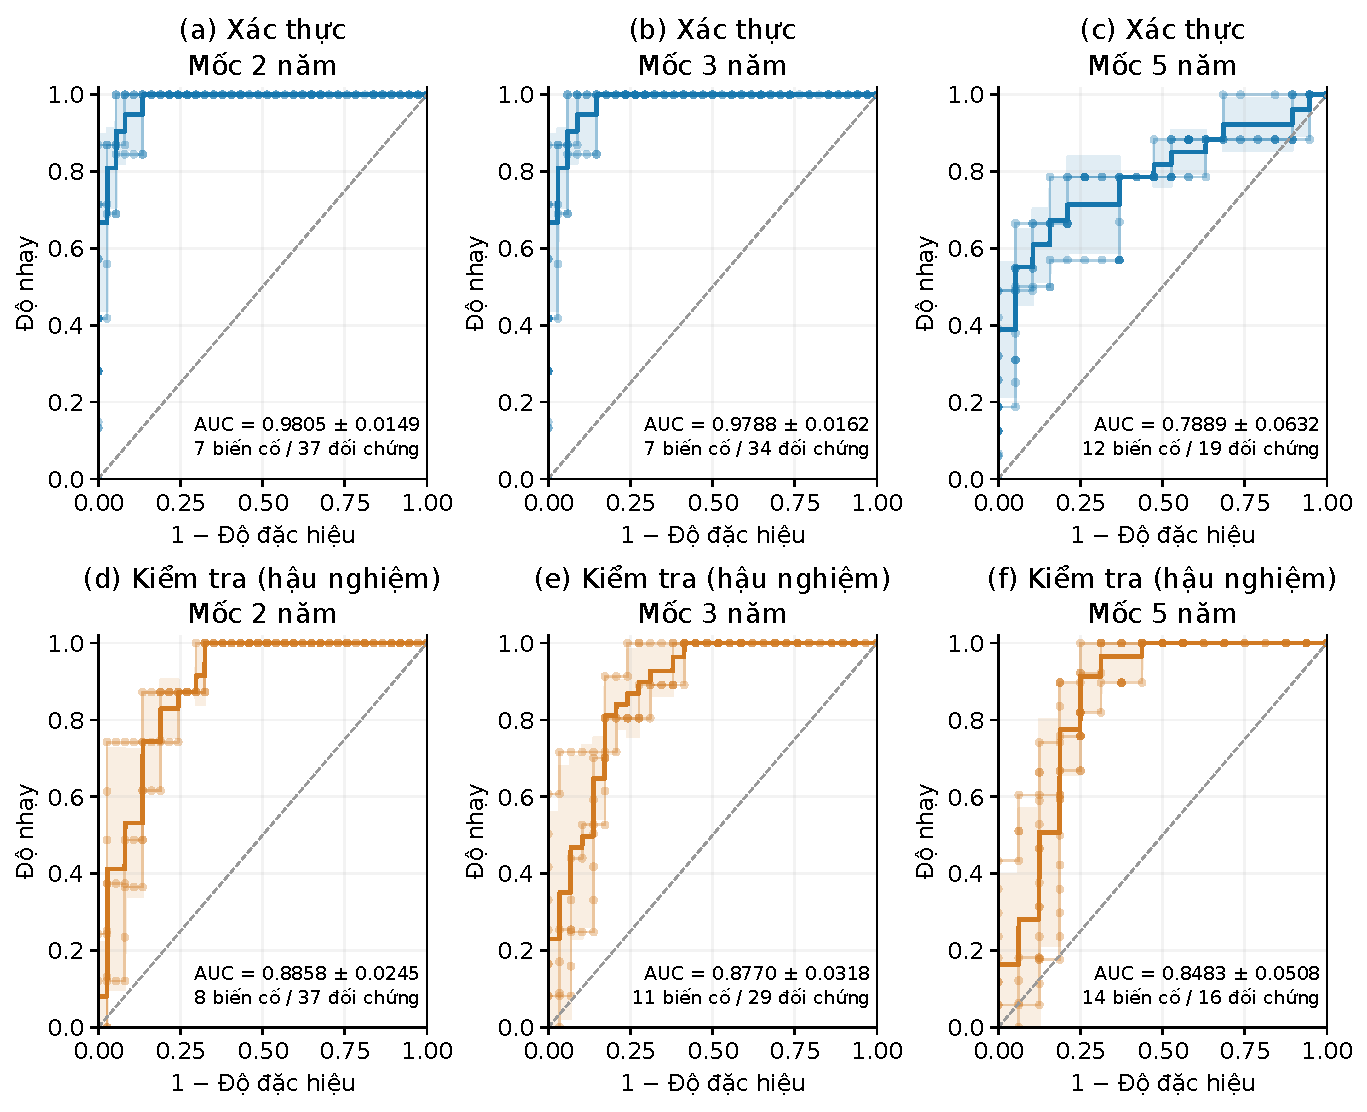
\includegraphics[width=\textwidth]{image/empirical-ipcw-roc.pdf}
\caption{Đường cong ROC có trọng số IPCW của RC-Free tại 2, 3 và 5 năm}
\label{fig:empirical-roc}
\captionsetup{justification=raggedright}
\caption*{Hàng trên: tập xác thực; hàng dưới: tập kiểm tra hậu nghiệm. Đường mảnh và chấm tròn là từng lần chạy; đường đậm là trung bình; vùng tô là $\pm1$ SD. Đường chéo biểu thị mức đoán ngẫu nhiên.}
\end{figure}

\clearpage
\subsection{Phân tầng Kaplan--Meier theo nhóm nguy cơ đồng thuận}
Hình~\ref{fig:survival-km} và Bảng~\ref{tab:km-statistics} đánh giá khả năng tách biệt hai nhóm nguy cơ cao và thấp (phân nhóm bằng ngưỡng trung vị tập huấn luyện và đồng thuận đa số qua ba lần chạy).

\begin{figure}[H]
\centering
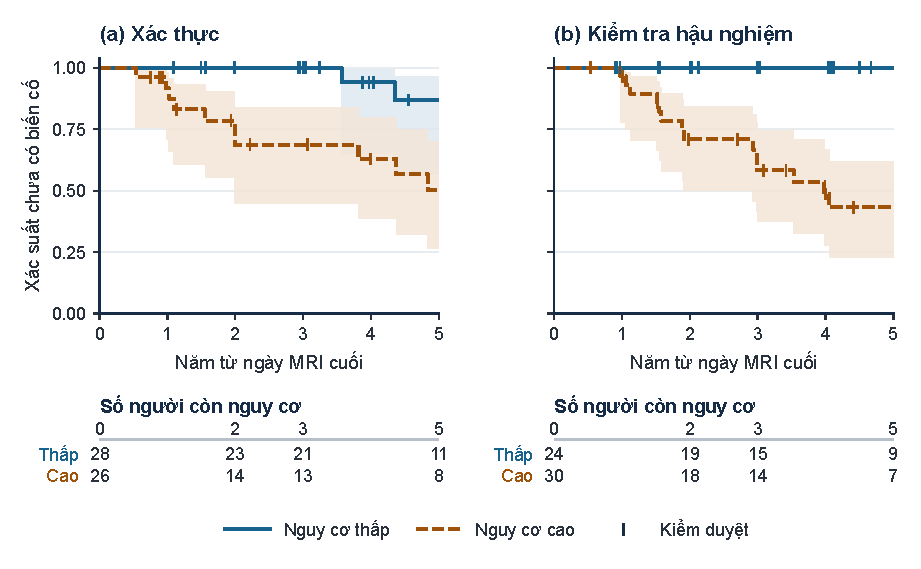
\includegraphics[width=\textwidth]{image/survival-km.pdf}
\caption{Đường cong Kaplan--Meier theo nhóm nguy cơ đồng thuận của RC-Free}
\label{fig:survival-km}
\captionsetup{justification=raggedright}
\caption*{Ô (a): tập xác thực; ô (b): tập kiểm tra hậu nghiệm. Vùng tô là khoảng tin cậy 95\%; dấu gạch dọc đánh dấu thời điểm kiểm duyệt. Bảng dưới trục hoành ghi số người còn nguy cơ tại các mốc thời gian.}
\end{figure}

\begin{table}[H]
\centering\small
\caption[Log-rank và HR theo nhóm nguy cơ]{Log-rank, HR cao/thấp và kiểm tra nguy cơ tỷ lệ (PH).}
\label{tab:km-statistics}
\begin{tabularx}{\linewidth}{@{}Y r r r r@{}}
\toprule
\textbf{Tập} & \textbf{Log-rank p} & \textbf{HR} & \textbf{CI 95\%} & \textbf{p (PH)} \\
\midrule
Xác thực & $0.013360$ & $3.79$ & $1.22$--$11.78$ & $0.103$ \\
Kiểm tra hậu nghiệm & $0.000313$ & $16.17$ & $2.12$--$123.17$ & $0.159$ \\
\bottomrule
\end{tabularx}
\end{table}


Hai đường cong tách biệt rõ nét trên cả hai tập dữ liệu, khẳng định năng lực phân tầng nguy cơ vượt trội của mô hình. Trên tập xác thực, nhóm nguy cơ thấp (28 người) chỉ ghi nhận 4 biến cố, trong khi nhóm nguy cơ cao (26 người) ghi nhận 12 biến cố — gấp ba lần nhóm thấp; kiểm định log-rank xác nhận sự khác biệt có ý nghĩa thống kê (\textbf{$p=0.0134$}), với tỷ số nguy cơ ước tính \textbf{HR = 3.79} (CI 95\%: 1.22--11.78). Trên tập kiểm tra hậu nghiệm, độ tương phản còn mạnh mẽ hơn: trong 24 người thuộc nhóm nguy cơ thấp gần như không ghi nhận ca suy giảm nào trong hơn 5 năm đầu (chỉ duy nhất 1 biến cố sau năm thứ năm), đối lập với 15 biến cố trong 30 người thuộc nhóm nguy cơ cao, đạt \textbf{log-rank $p<0.001$} và \textbf{HR = 16.17} (CI 95\%: 2.12--123.17). Khoảng tin cậy rộng của HR trên tập kiểm tra bắt nguồn trực tiếp từ việc nhóm nguy cơ thấp chỉ có đúng một biến cố làm mẫu số so sánh; ngay cả cận dưới của khoảng tin cậy 95\% vẫn đạt 2.12, cho thấy nhóm nguy cơ cao vẫn có tốc độ tiến triển cao hơn rõ rệt. Đồng thời, phép kiểm tra phần dư Schoenfeld cho $p=0.1031$ trên tập xác thực và $p=0.1592$ trên tập kiểm tra (đều lớn hơn 0.05), chứng tỏ tỷ lệ nguy cơ giữa hai nhóm duy trì ổn định theo thời gian và khẳng định RC-Free là kiến trúc vừa đạt hiệu quả xếp hạng cao nhất, vừa cho khả năng phân tầng sống còn sắc nét và tin cậy nhất trong toàn bộ các thử nghiệm.

\section{Trả lời các câu hỏi nghiên cứu}
\label{sec:rq-results}
Tổng hợp toàn bộ chuỗi thực nghiệm trên, câu trả lời cho năm câu hỏi nghiên cứu ở Bảng~\ref{tab:rq} như sau:

\begin{description}[leftmargin=1.35cm,labelwidth=1.1cm,itemsep=.3em]
\item[RQ1.] \emph{Dữ liệu dọc}: Chuỗi ba lần chụp MRI cải thiện rõ rệt so với chỉ dùng ảnh cuối khi kết hợp T-LSTM với attention, tăng C-index xác thực từ 0.7333 lên \textbf{0.7833} (Bảng~\ref{tab:exploratory}).
\item[RQ2.] \emph{Đa phương thức}: Bổ sung radiomics và dữ liệu lâm sàng bằng ghép nối tiếp tục nâng C-index xác thực lên \textbf{0.8125} (+0.0292 so với chỉ dùng MRI, Bảng~\ref{tab:exploratory}).
\item[RQ3.] \emph{Tương tác cặp so với ghép nối}: Khi giữ cùng trọng số khởi tạo cho các phần chung, phép tích ngoài đạt C-index xác thực trung bình cao hơn ghép nối \textbf{0.0135} (0.8285 so với 0.8149, Bảng~\ref{tab:matched-fusion}).
\item[RQ4.] \emph{Phân rã CP}: CP giảm \textbf{98.38\%} số tham số ở ba lớp song tuyến đầu (90.90\% ở ba khối tương tác; 0.67\% toàn mạng, Bảng~\ref{tab:interaction-parameters}), đổi lại mức giảm nhỏ 0.0066 C-index giữa Full CP và Full Outer-Product (Bảng~\ref{tab:standard-bench}).
\item[RQ5.] \emph{Tinh gọn thành RC-Free}: Khả thi và hiệu quả. Bỏ cặp RC tiết kiệm thêm \textbf{15460 tham số} so với Full CP, rút từ sáu xuống bốn nhánh và đạt C-index xác thực trung bình cao nhất trong bảy cấu trúc CP (\textbf{0.8347}, Bảng~\ref{tab:new-topology}), đồng thời phân tầng nguy cơ có ý nghĩa thống kê trên đường cong Kaplan--Meier (Bảng~\ref{tab:km-statistics}).
\end{description}
